\section{twilight}
\begin{theorem}\label{theorem:twilight}
    the solution problem is not in NP.
\end{theorem}

\begin{figure}\label{figure:twilight-constructs}
  \mbox{
    \subfigure[clock]{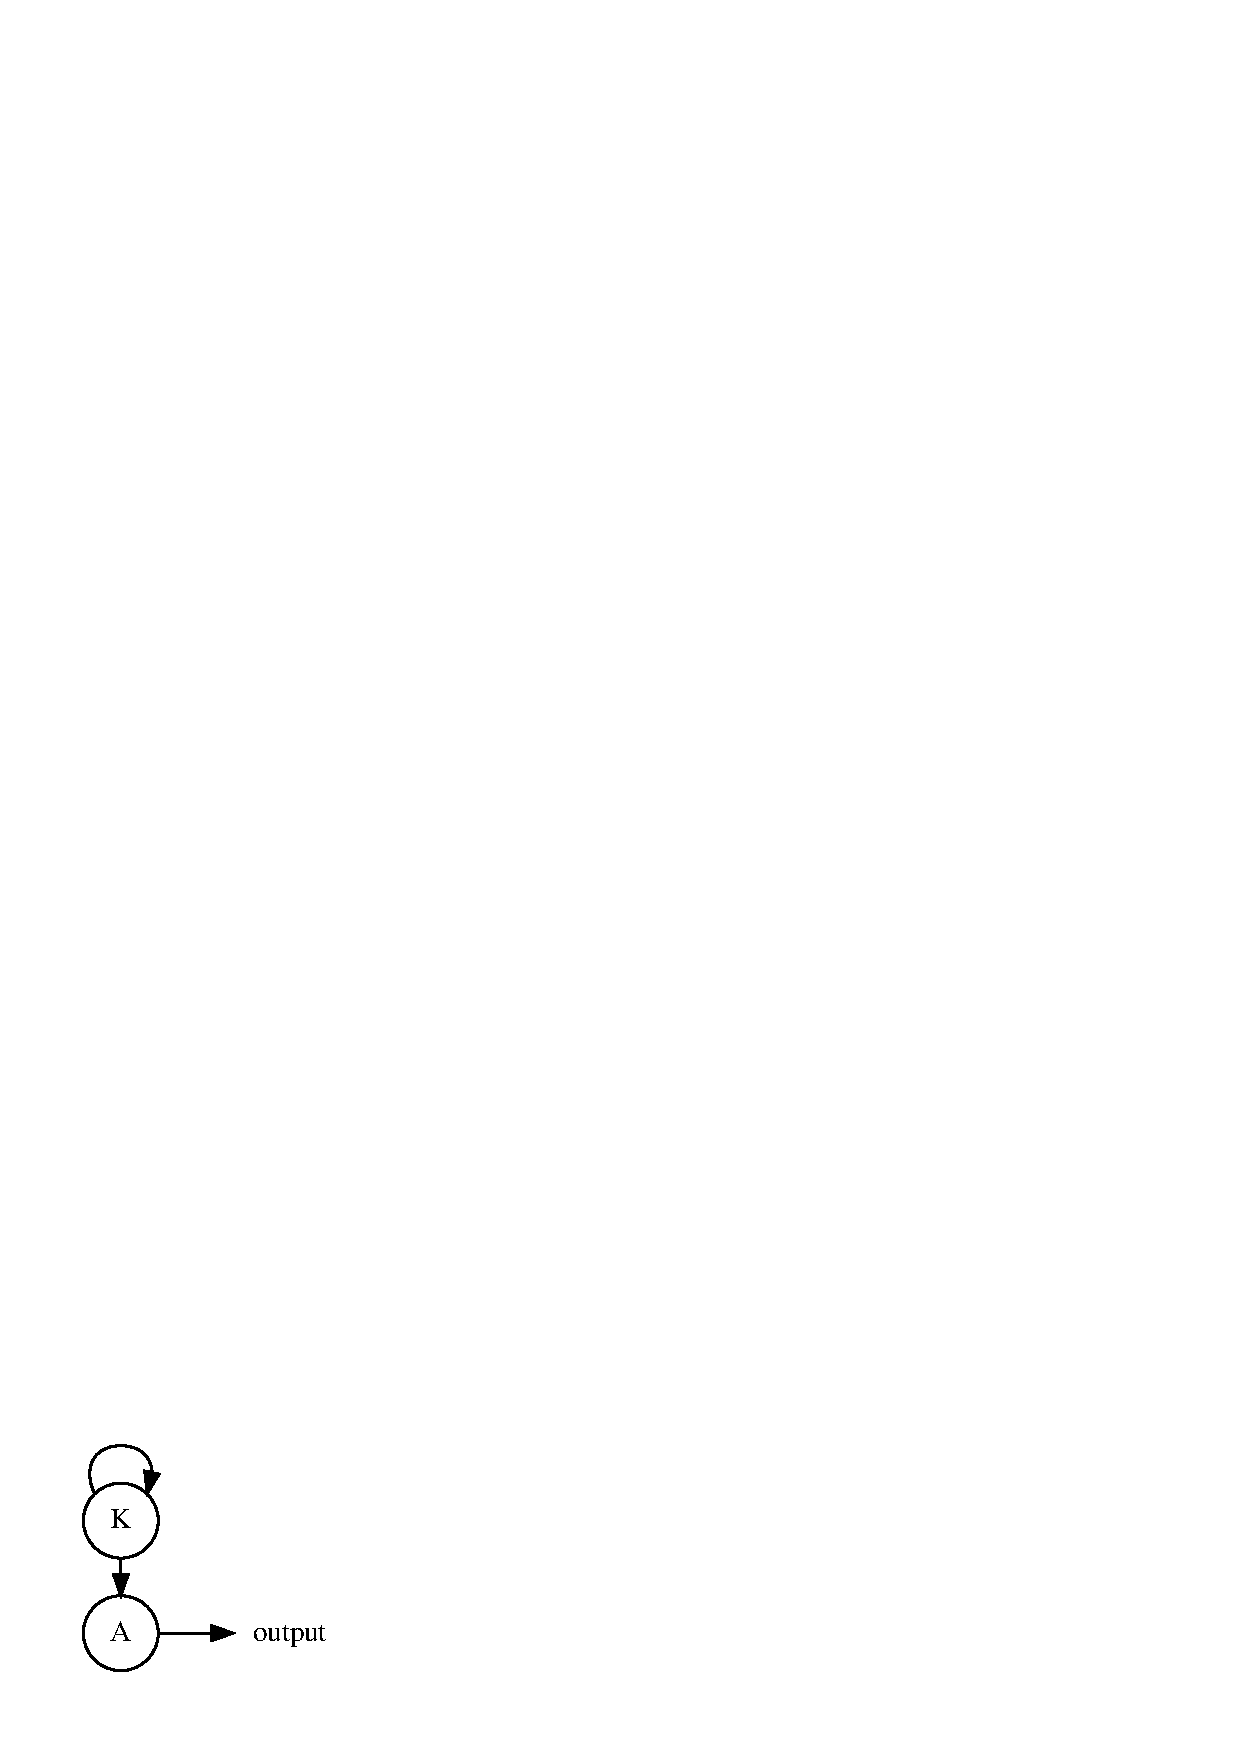
\includegraphics[width=0.30\textwidth]{image/a.dot.pdf}}\label{twilight-construct:clock}
    \subfigure[register]{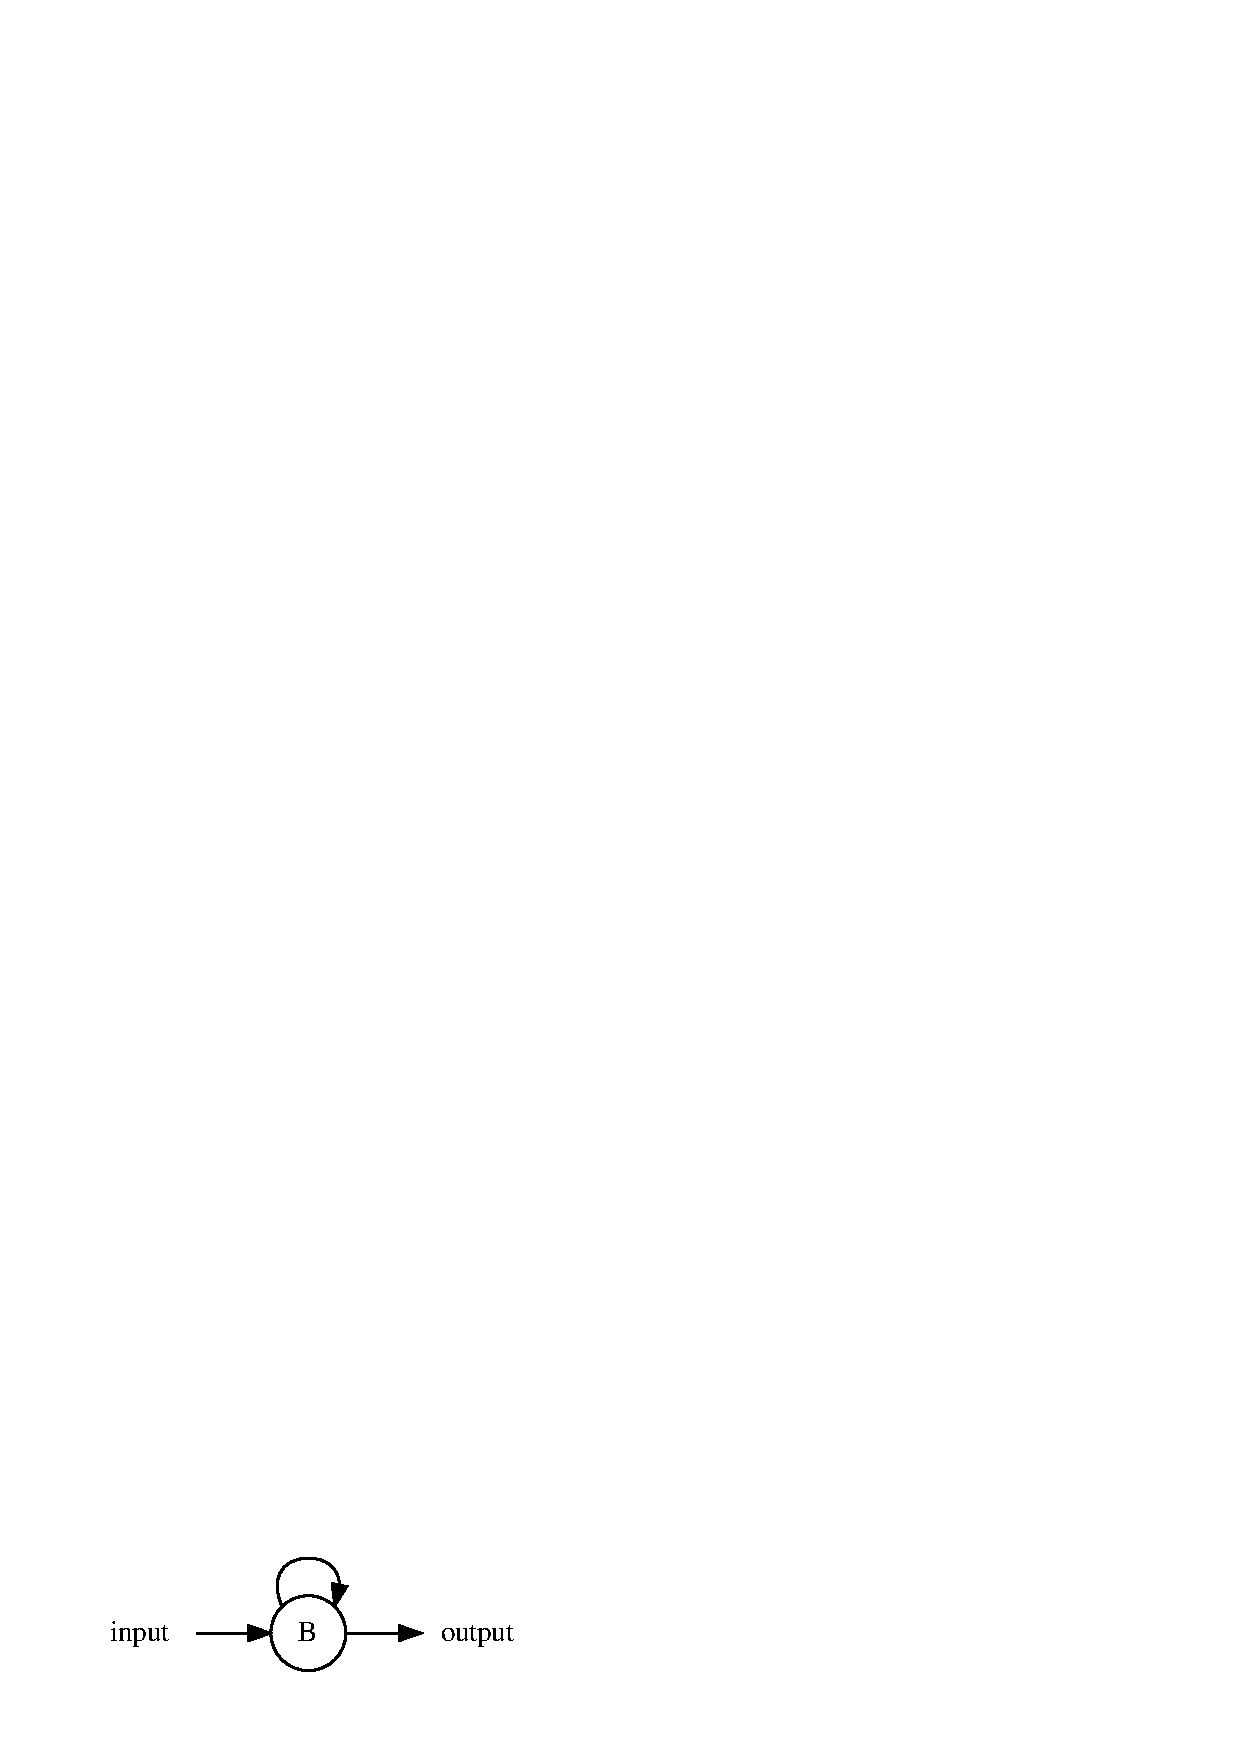
\includegraphics[width=0.30\textwidth]{image/b.dot.pdf}}\label{twilight-construct:register}
    \subfigure[carry]{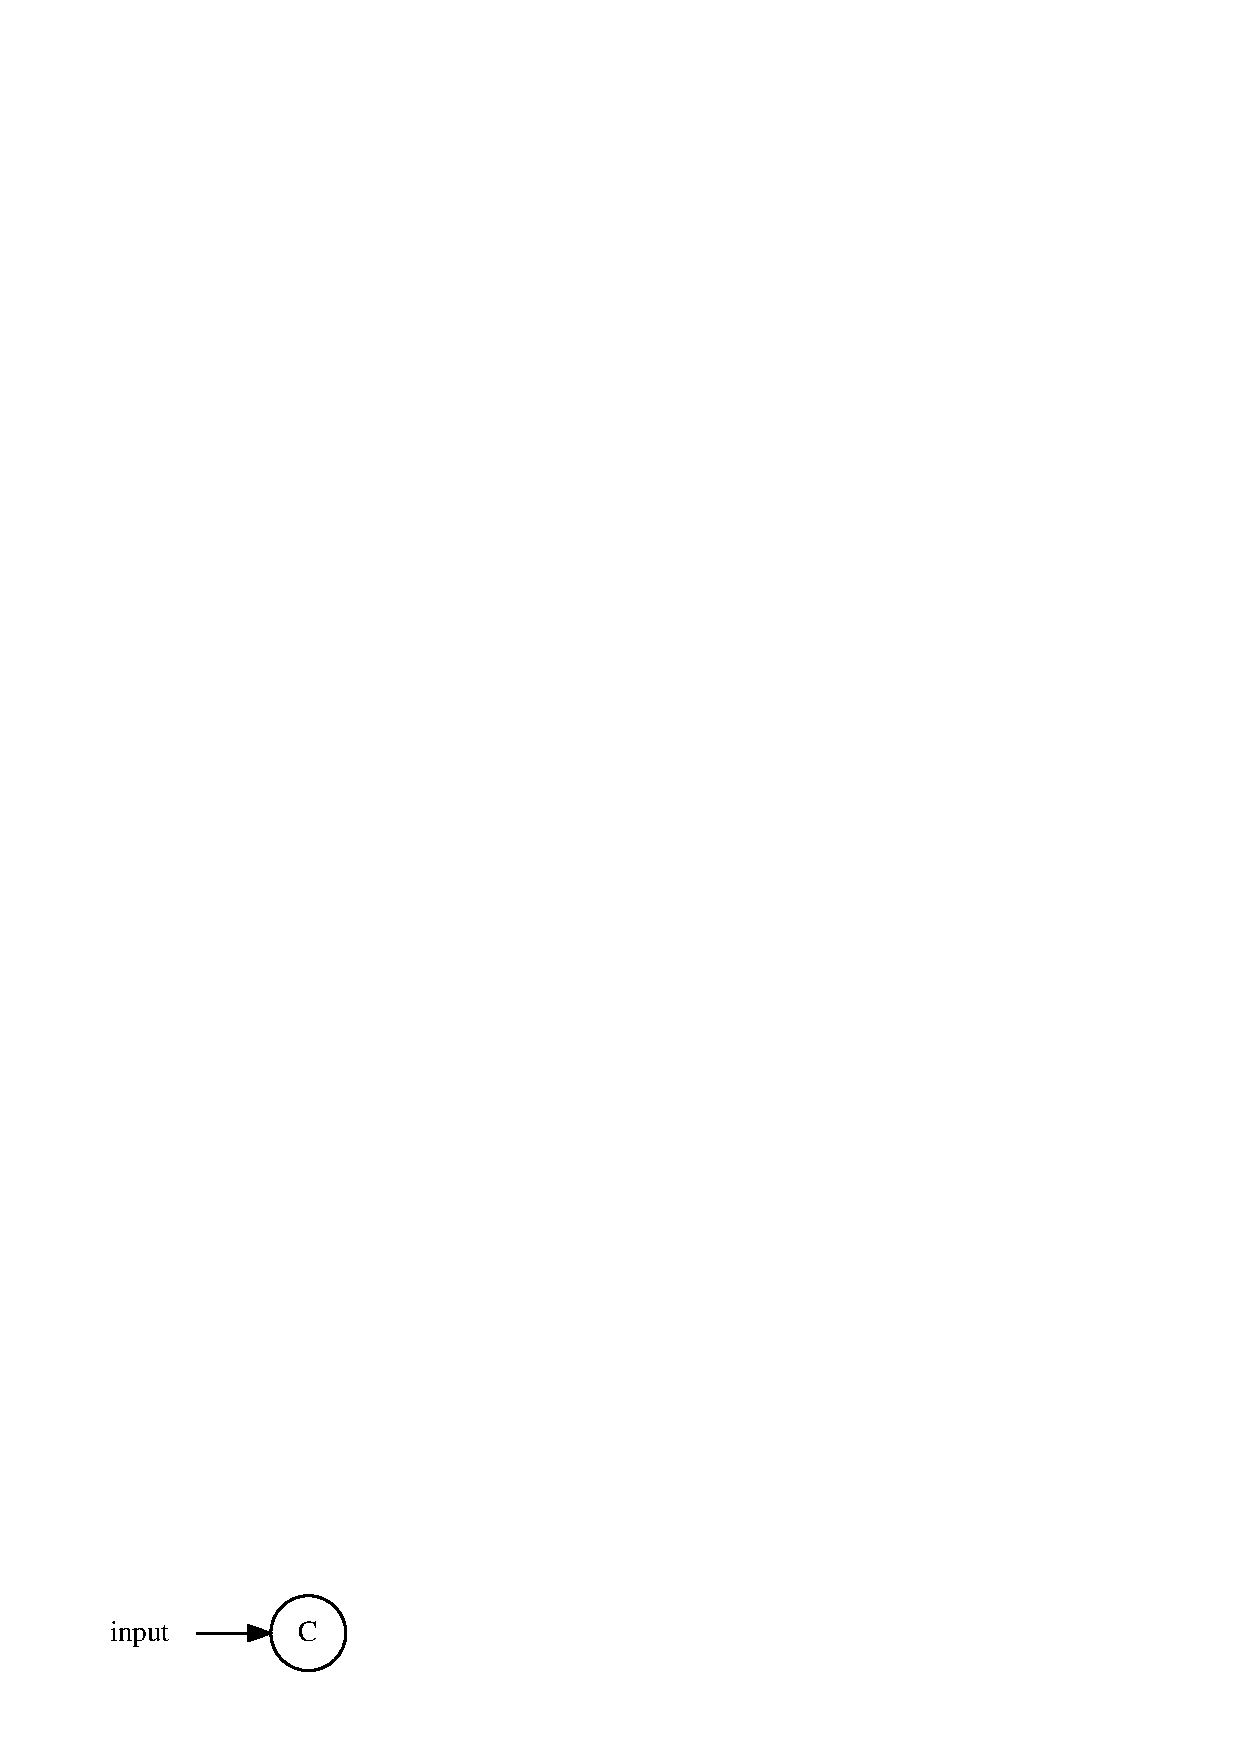
\includegraphics[width=0.30\textwidth]{image/c.dot.pdf}}\label{twilight-construct:carry}
   }
  \caption{twilight constructs}
\end{figure}

Take a look at figure \ref{figure:twilight-constructs}. It displays various constructs used in the proof of theorem \ref{theorem:twilight}.

Construct \ref{twilight-construct:clock} is called a clock. It has two vertices, which are both in the \emph{active} state. The top vertex can be used to kill the clock. Pressing it will change the state of the clock vertices to 0, which is an \emph{inactive} state.
The bottom vertex of the clock construct will send a signal through the output edge. This signal can be used to increment the vertex that will be connected to it. 

Construct \ref{twilight-construct:register} of figure \ref{figure:twilight-construct} is called a register. It consist of a sole vertex connected to the input and output. Initially this vertex is in the state 0. It takes at least $q-1$ input signals before the \emph{register} construct can pass a signal to its output.

The last construct, \ref{twilight-construct:carry} is called a carry. It is a sole vertex connected to the input. Initially the carry vertex is in state 1. Since it is only influenced by the input, it needs $q-1$ input signals before it is turned off.

\begin{figure}
  \includegraphics{image/p3.dot.pdf}
  \caption{Problem $P_{3}$}\label{figure:p3}
\end{figure}

With these constructs we will define a family of problems $\left(P_{n}\right)_{n=0}^{\infty}$. To define our family we introduce a little notation. $a$ will denote a clock construct, $b$ denotes a register and $c$ denotes a carry. Concatenation $uv$ of verbs $u$ and $v$ means to connect the output of $u$ to the input of $v$. Exponentiation will be interpreted as iterated concatenation.

With these conventions it is easy to describe our family: $P_{n} := ab^{n}c$. In figure \ref{figure:p3} you see a depiction of $P_{3}$.

The crux of the proof of theorem \ref{theorem:twilight} can be found in the following lemma.

\begin{lemma}
  For construct $b^{n}$ there need to be at least
  \[\frac{(q-1)^{n+1} - 1}{q-2}\]
  presses before an output signal occurs.
\end{lemma}

\begin{proof}
  We will prove this with induction on the size of the construct. Notice that for $n=0$ the input is directly coupled to the output so each input signal corresponds to one output signal, in accordance with lemma.

  Take a look at construct $b$. Each input signal changes the state of the vertex from $i \mapsto i+1$. In order for the vertex to reach state $q-1$ we need at least $q-1$ input signals. Before an output signal is send the vertex of $b$ should be pressed. This sets the least amount of presses to send an output signal to $(q-1) + 1$ which equals $\frac{(q-1)^2 - 1}{q-2}$.

  Now assume that construct $b^{k}$ needs at least $\frac{(q-1)^{k+1} - 1}{q-2}$ input signals before an output signal occurs. We will show that the construct $b^{k+1}$ will need at least $\frac{(q-1)^{k+1} - 1}{q-2}$ input signal.

  Since $b^{k+1} = b^{k}b$ and we know that $b$ needs $q-1$ input signals to reach state $q-1$ before we can press its vertex to produce an output signal, we have for the least amount of presses for $b^{k+1}$

  \[
    \left(\frac{(q-1)^{k+1} - 1}{q-2}\right)(q-1) + 1 =
    \frac{(q-1)^{k+2} - (q-1)}{q-2} + \frac{q-2}{q-2} = 
    \frac{(q-1)^{k+2} - 1}{q-2}
  \]

  Proving our lemma.
\end{proof}

The crux can be used in the following theorem

\begin{theorem}
  The problem $P_{n}$ needs $\frac{(q-1)^{n+2} - 1}{q-2}$ presses to solve.
\end{theorem}

\begin{proof}
  Note that $P_{n} = ab^nc$. $c$ needs $(q-1)$ input signals to transistion from $1$ to $0$. These need to be delivered by $b^{n}$, which by the preceding lemma, needs at least $\frac{(q-1)^{n+1} - 1}{q-2}$ presses. Afterwards we need to kill the clock which can be achieved with one press of the kill switch.
  
  So the least number of presses to solve $P_{n}$ is $\frac{(q-1)^{n+1} - 1}{q-2}(q-1) + 1 = \frac{(q-1)^{n+2} - 1}{q-2}$.
\end{proof}

The proof of theorem \ref{theorem:twilight} is a consequence

\begin{proof}
  $|P_{n}| = |ab^{n}c| = |a| + |b^{n}| + |c| = 2 + n + 1 = n + 3$. By the preceding family the solution length is not bounded by a polynomial in the number of vertices.
\end{proof}